\chapter{Convolution}
\doublespacing

\begin{definition}
	The \textbf{convolution} $*$, of two functions $F$ and $G$ is defined as:
	\begin{equation}
		(F*G)(t) = \int_{-\infty}^\infty F(t) \;G(t - \tau) \; d\tau
	\end{equation}
\end{definition}

Is often visualized by graphically flipping one function and sliding it across the other as seen in Figure \ref{convolution}.

\begin{figure}[h]
\label{convolution}
\caption[Convolution of box signal with itself]{The convolution of the box signal 
$f(t)=g(t)=\left( 0^\oiOpOp{-\infty,-0.5} \oplus 1^\oiClCl{-0.5,0.5} \oplus 0^\oiOpOp{0.5,\infty} \right)$ with itself.
\emph{(from wikipedia; need to create new versions)}}
\centering
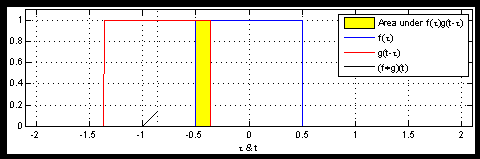
\includegraphics[scale=0.6]{diagrams/conv1}
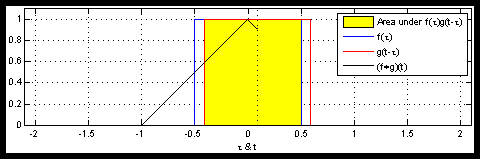
\includegraphics[scale=0.6]{diagrams/conv2}
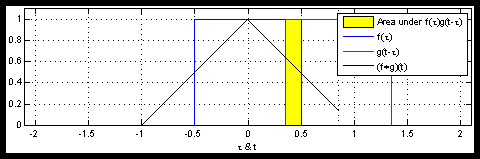
\includegraphics[scale=0.6]{diagrams/conv3}
\end{figure}

Has applications in signal processing

Frequently used in image processing

  Gaussian blurring result of convolving a function with the Gaussian function:
\begin{equation}
	f(x) = a \; \text{exp} \left( - \frac{(x-b)^2}{2c^2} \right)
\end{equation}

In statistics a weighted moving average is a convolution

\section{Convolution of Piecewise Functions}

We are interested in \emph{Symbolic Linear Convolution} (of piecewise continuous functions)

First we consider the convolution of ``one piece'' functions:

\begin{equation}
	F(x)=f^{[a_f,b_f)}(x) = 
		\begin{cases}
			f(x) & a_f \leq x < b_f \\
			0 & \text{otherwise}
		\end{cases}
\end{equation}

\begin{equation}
	G(x)=g^{[a_g,b_g)}(x) = 
		\begin{cases}
			g(x) & a_g \leq x < b_g \\
			0 & \text{otherwise}
		\end{cases}
\end{equation}

Generally we assume that $b_f - a_f \leq b_g - a_g$, ($f$ is shorter)

If this is not the case, convolution is commutative so we simply rearrange: $F * G = G * F$

\begin{align}
	(F*G)(t) 
	&= \int_{-\infty}^\infty F(\tau)\; G(t-\tau) \; d\tau \notag \\
	&= \int_{a_f}^{b_f} f(\tau) \; G(t-\tau) \; d\tau \notag \\
	&= 	\begin{cases}
			\int_{a_f}^{x-a_g} f(\tau) \; g(t-\tau) \; d\tau 	& (a_f+a_g) \leq t < (b_f+a_g) \\
			\int_{a_f}^{b_f} f(\tau) \; g(t-\tau) \; d\tau		& (b_f+a_g) \leq t < (a_f+b_g) \\
			\int_{x-b_g}^{b_f} f(\tau) \; g(t-\tau) \; d\tau	& (a_f+b_g) \leq t < (b_f+b_g) \\
			0										& \text{otherwise}
		\end{cases}
\end{align}


This is the way it's typically done.

\section{Hybrid Function Convolution}

With hybrid functions we do not have to worry about the relative length of $f$ and $g$ intervals.

Instead for hybrid functions $F = f^{[a_f, b_f)}$ and $G = g^{[a_f, b_f)}$:

\begin{align}
	(F \;*\; G) (t) = 
		\mathcal{R}_+ &\left( \; \left( 
			\int_{a_f}^{x-a_g} f(\tau) \; g(t-\tau) \; d\tau \right)^{[\![a_f+a_g,\; b_f+a_g)\!)} 
				\right. \notag \\ &\oplus \left( 
			\int_{a_f}^{b_f} f(\tau) \; g(t-\tau) \; d\tau \right)^{[\![b_f+a_g,\; a_f+b_g)\!)} 
				\notag \\ &\oplus \left. \left( 
			\int_{x-b_g}^{b_f} f(\tau) \; g(t-\tau) \; d\tau \right)^{[\![a_f+b_g,\; b_f+b_g)\!)} 
				\; \right)(t)
\end{align}

When $b_f - a_f \leq b_g - a_g$ then the intervals will be disjoint and the expression is identical to 2.61

Otherwise, the interval $[\![b_f +a_g, \; a_f + b_g)\!)$ will have a negative orientation.

For $(a_f+b_g) \leq t < (b_f+a_g)$ then $t$ will be in all three regions and we have


\section{Infinite Intervals}


\section{Example}

\newpage